% Generated by thesis/ch7/exp1/networks.py -- do not edit by hand.
\ifdefined\netfigheight\else\newlength{\netfigheight}\setlength{\netfigheight}{0.9\textwidth}\fi
\begin{sidewaysfigure}
  \centering
  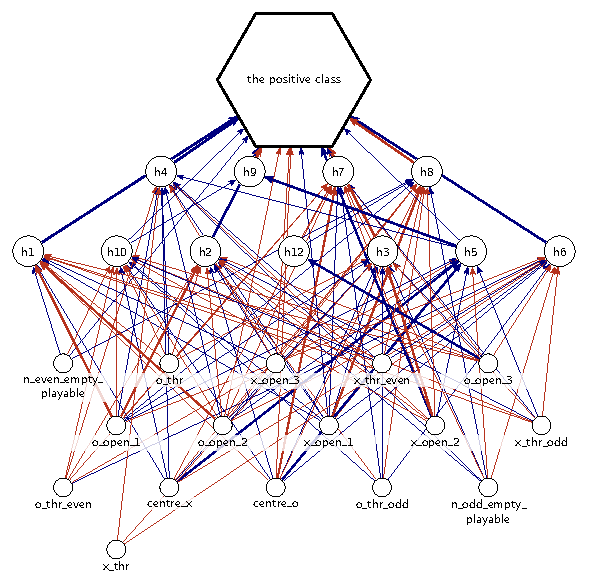
\includegraphics[width=\textheight,height=\netfigheight,keepaspectratio]{figures/exp1/networks/c4lf-lines-heavy-s0-raw}
  \caption{Connect-4, lines, seed 0: the network as trained, before any explanation. Bottom: the input columns; circles h1, h2, \ldots: hidden units; hexagon: the output. Edges: blue, a positive weight (raises the score); red, a negative weight (lowers it); thicker, a larger weight. Double outline: acts at a fixed rate everywhere (dashed double: on the observed data).}
  \label{fig:exp1-net-c4lf-lines-heavy-s0-raw}
\end{sidewaysfigure}
